\documentclass{article}
\usepackage{graphicx} % Required for inserting images
\usepackage{xcolor}
\usepackage{listings}
\usepackage{float}
\usepackage{amsmath}
\usepackage{amssymb}

\definecolor{codebg}{RGB}{245,245,245}
\definecolor{codetext}{RGB}{36,41,46}
\definecolor{codekeyword}{RGB}{0,92,197}
\definecolor{codestring}{RGB}{163,21,21}
\definecolor{codecomment}{RGB}{106,153,85}
\definecolor{codenumber}{RGB}{30,60,120}
\definecolor{class0}{HTML}{66C2A5}
\definecolor{class1}{HTML}{FC8D62}
\definecolor{class2}{HTML}{8DA0CB}
\definecolor{class3}{HTML}{FFD92F}

\lstset{
    backgroundcolor=\color{codebg},
    basicstyle=\ttfamily\small\color{codetext},
    keywordstyle=\color{codekeyword}\bfseries,
    stringstyle=\color{codestring},
    commentstyle=\color{codecomment}\itshape,
    numberstyle=\tiny\color{codenumber},
    numbers=left,
    numbersep=8pt,
    frame=single,
    rulecolor=\color{codebg},
    framerule=0.5pt,
    showstringspaces=false,
    tabsize=4,
    breaklines=true
}

\title{EEN245 A1}
\author{Vansh Agrawal \and Ayush Ahuja}
\date{January 2026}

\begin{document}

\maketitle

\section{Part A: PyG basics}
The code is attached in Listing 1 in the appendix.
\begin{itemize}
    \item Number of nodes: 34.
    \item Number of edges: 156.
    \item Shape of \texttt{data.x}: 34x34.
    \item Shape of \texttt{data.\allowbreak edge\_index}: 2x154.
    \item Number of node labels: 4.
\end{itemize}

\noindent \texttt{data.x} is a matrix of number of nodes times the number of features. Each row corresponds to the values of that node for each feature. 
\texttt{data.\allowbreak edge\_index} is a 2 by number of edges sized matrix. The first row of the ith column represents the start point of the Ayat edge and the second row of the Ayat column represents the end point of the ith edge.
\texttt{data.y} is the actual value which we want to train on. It can be for edges or nodes or the entire graph. We hide a part of \texttt{data.y} to be able to test our model and train it on the remaining part.

\section{Part B: Visualizing the graph}
\begin{figure}[H]
    \centering
    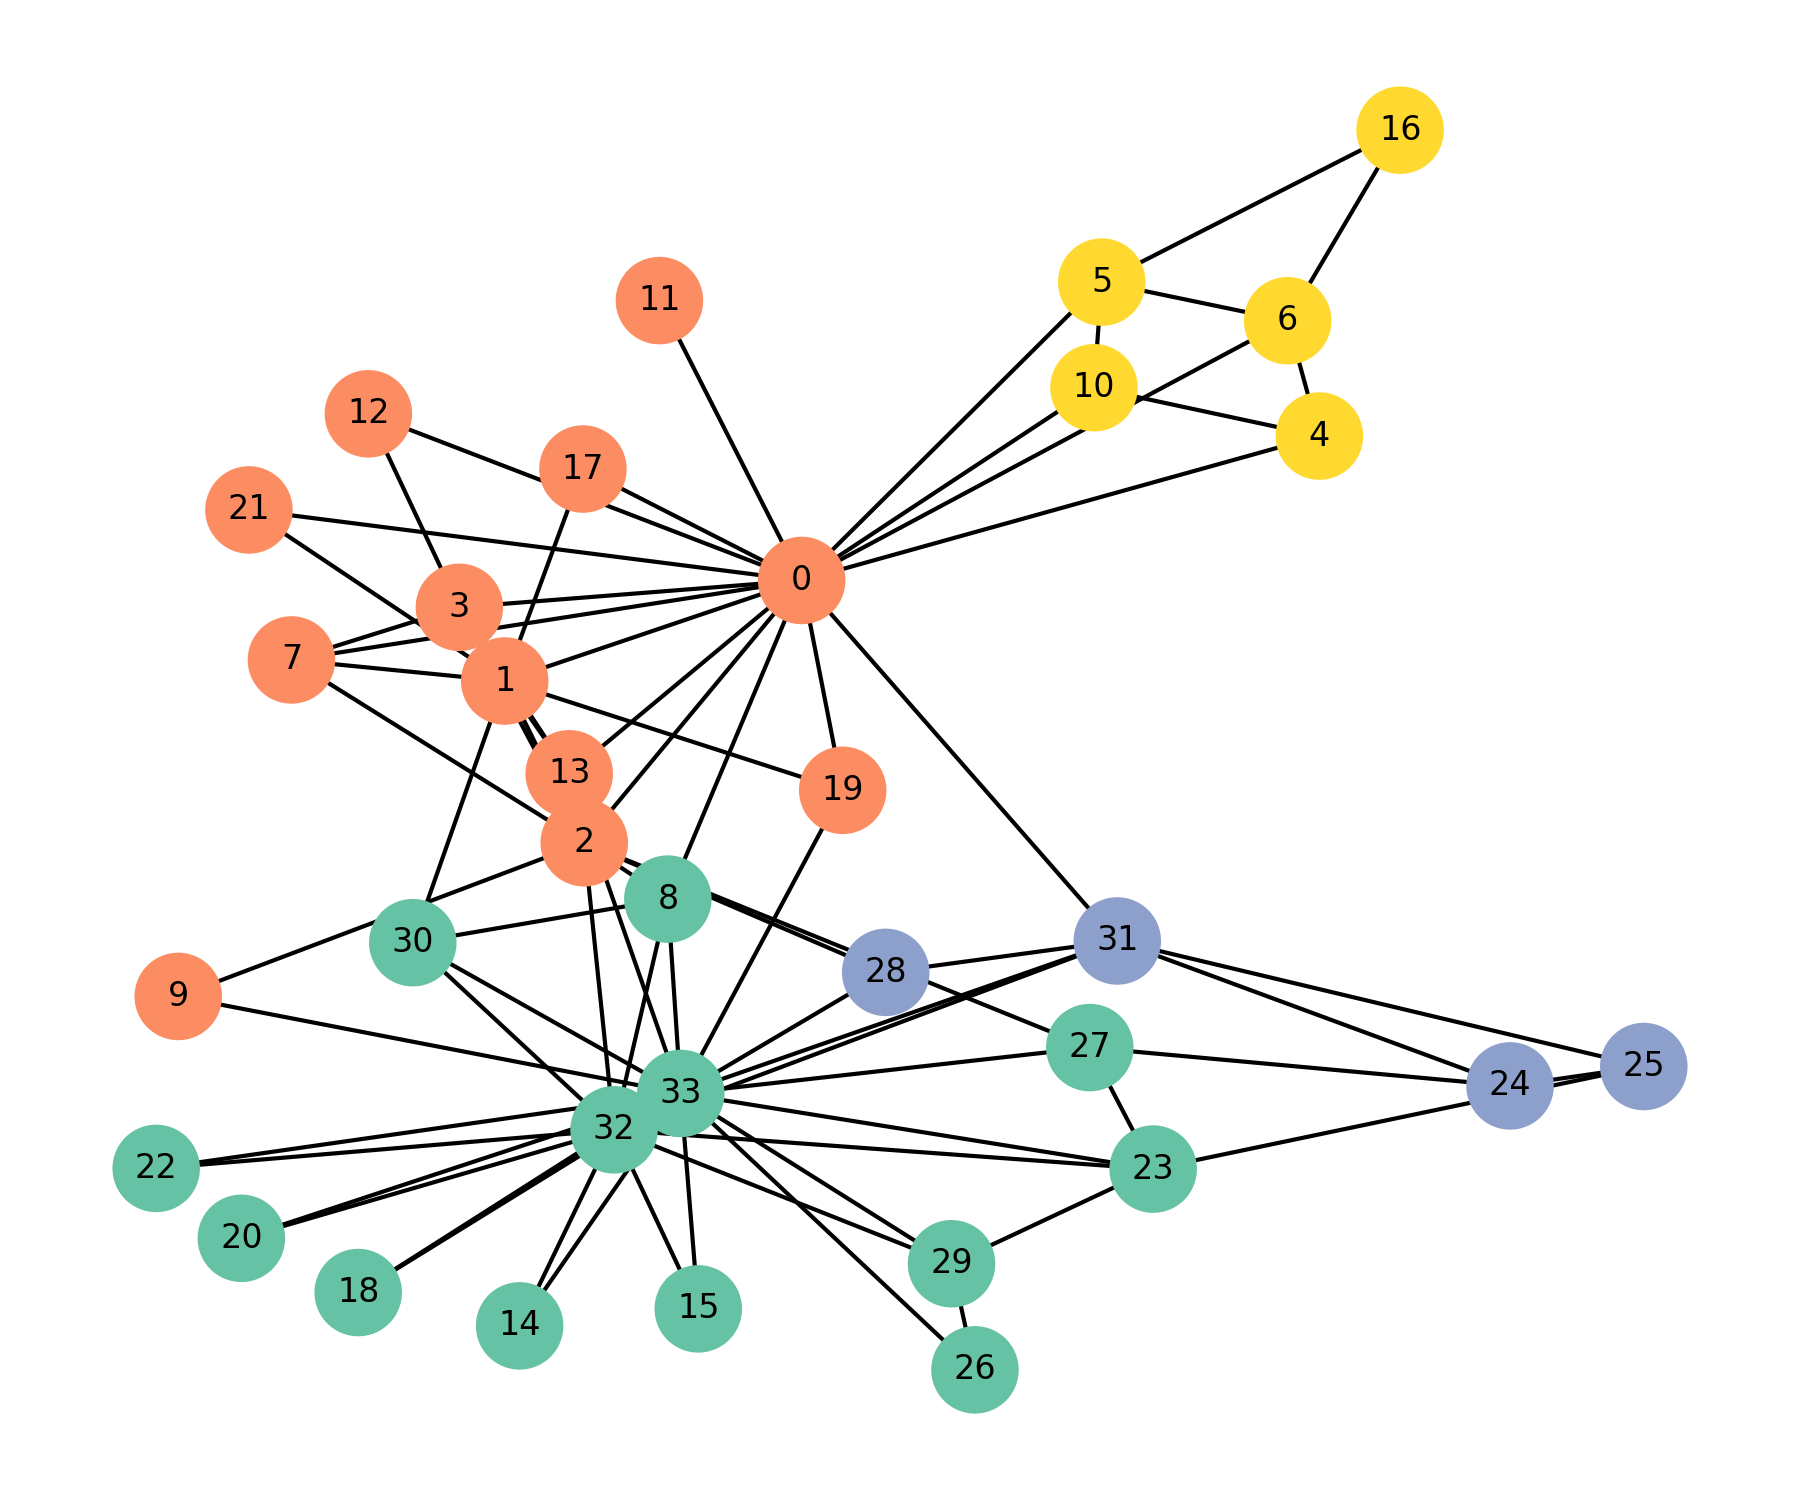
\includegraphics[width=0.85\linewidth]{karate_club_graph.png}
    \vspace{0.5em}

    \begin{tabular}{llll}
        \colorbox{class0}{\strut\hspace{1em}}~Class 0 &
        \colorbox{class1}{\strut\hspace{1em}}~Class 1 &
        \colorbox{class2}{\strut\hspace{1em}}~Class 2 &
        \colorbox{class3}{\strut\hspace{1em}}~Class 3
    \end{tabular}
    \caption{Visualized graph: each color stands for a class.}
\end{figure}

\section{Part C: Structural feature embeddings}
\subsection{C1. Structural features}
We compute six structural features per node: degree, betweenness centrality, closeness centrality, PageRank, eigenvector centrality, and clustering coefficient. For each feature we build a vector ordered by node index (0 to $N-1$), then stack these vectors column-wise to obtain $X_{\text{struct}} \in \mathbb{R}^{N \times 6}$. Finally, we normalize each feature with z-score normalization (subtract mean and divide by standard deviation) to place all features on a comparable scale. The implementation is included in Listing 3 in the appendix.
\subsection{C2. Visualize structural embeddings}
We take the normalized structural feature matrix from C1 and reduce it to 2D using PCA. The 2D points are then plotted and colored by the node labels. The visualization is shown in Figure~\ref{fig:struct_pca} and the code is in Listing 4.

\begin{figure}[H]
    \centering
    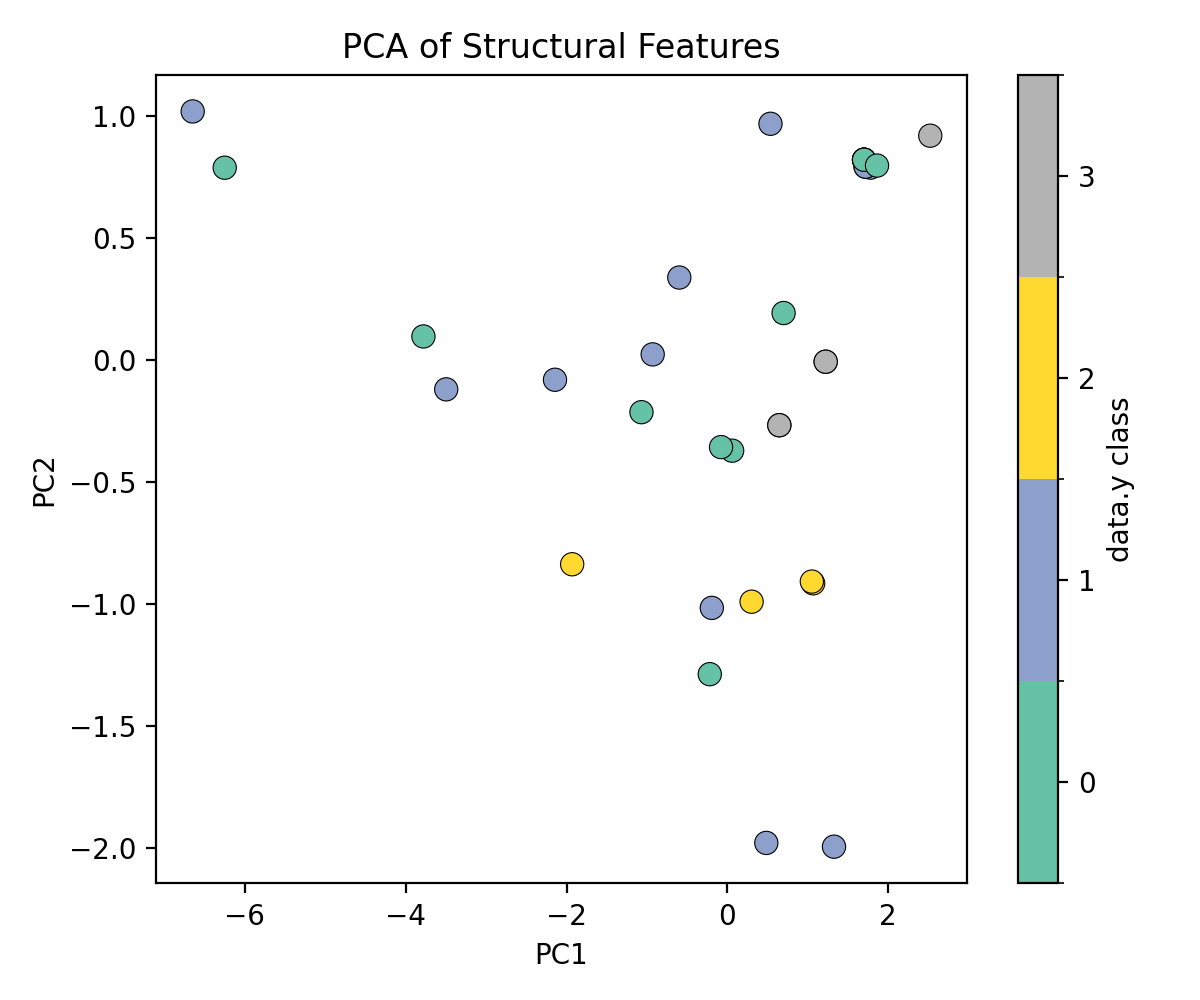
\includegraphics[width=0.75\linewidth]{structural_pca.png}
    \caption{PCA of structural features; colors indicate the node labels.}
    \label{fig:struct_pca}
\end{figure}

\subsection{C3. Node classification using structural features}
We train two simple classifiers on $X_{\text{struct}}$ (6 structural features per node): a 2-layer MLP (6 $\rightarrow$ 16 $\rightarrow$ 4) and logistic regression. We evaluate both using stratified 5-fold cross-validation (seed 42). The mean test accuracies are:
\begin{itemize}
    \item \textbf{MLP:} \textbf{56.19\%} $\pm$ \textbf{17.41\%} (mean train accuracy 100\%).
    \item \textbf{Logistic Regression:} \textbf{44.29\%} $\pm$ \textbf{9.48\%} (mean train accuracy 79.42\%).
\end{itemize}
The implementation is shown in Listing~\ref{lst:c3}.

\section{Part D: Node classification using node features}
\subsection{D1. Node classification using node features only}
We train the same two classifiers (MLP and logistic regression) on the raw node features $X = \texttt{data.x}$ and evaluate them with stratified 5-fold cross-validation (seed 42). The mean test accuracies are:
\begin{itemize}
    \item \textbf{MLP:} \textbf{35.71\%} $\pm$ \textbf{9.04\%} (mean train accuracy 100\%).
    \item \textbf{Logistic Regression:} \textbf{29.52\%} $\pm$ \textbf{1.90\%} (mean train accuracy 100\%).
\end{itemize}
The implementation is shown in Listing~\ref{lst:d1}.

\subsection{D2. Visualize node features}
We reduce the node features to 2D using PCA and color by node labels. The visualization is shown in Figure~\ref{fig:node_feat_pca} and the code is provided in Listing~\ref{lst:d2}.

\begin{figure}[H]
    \centering
    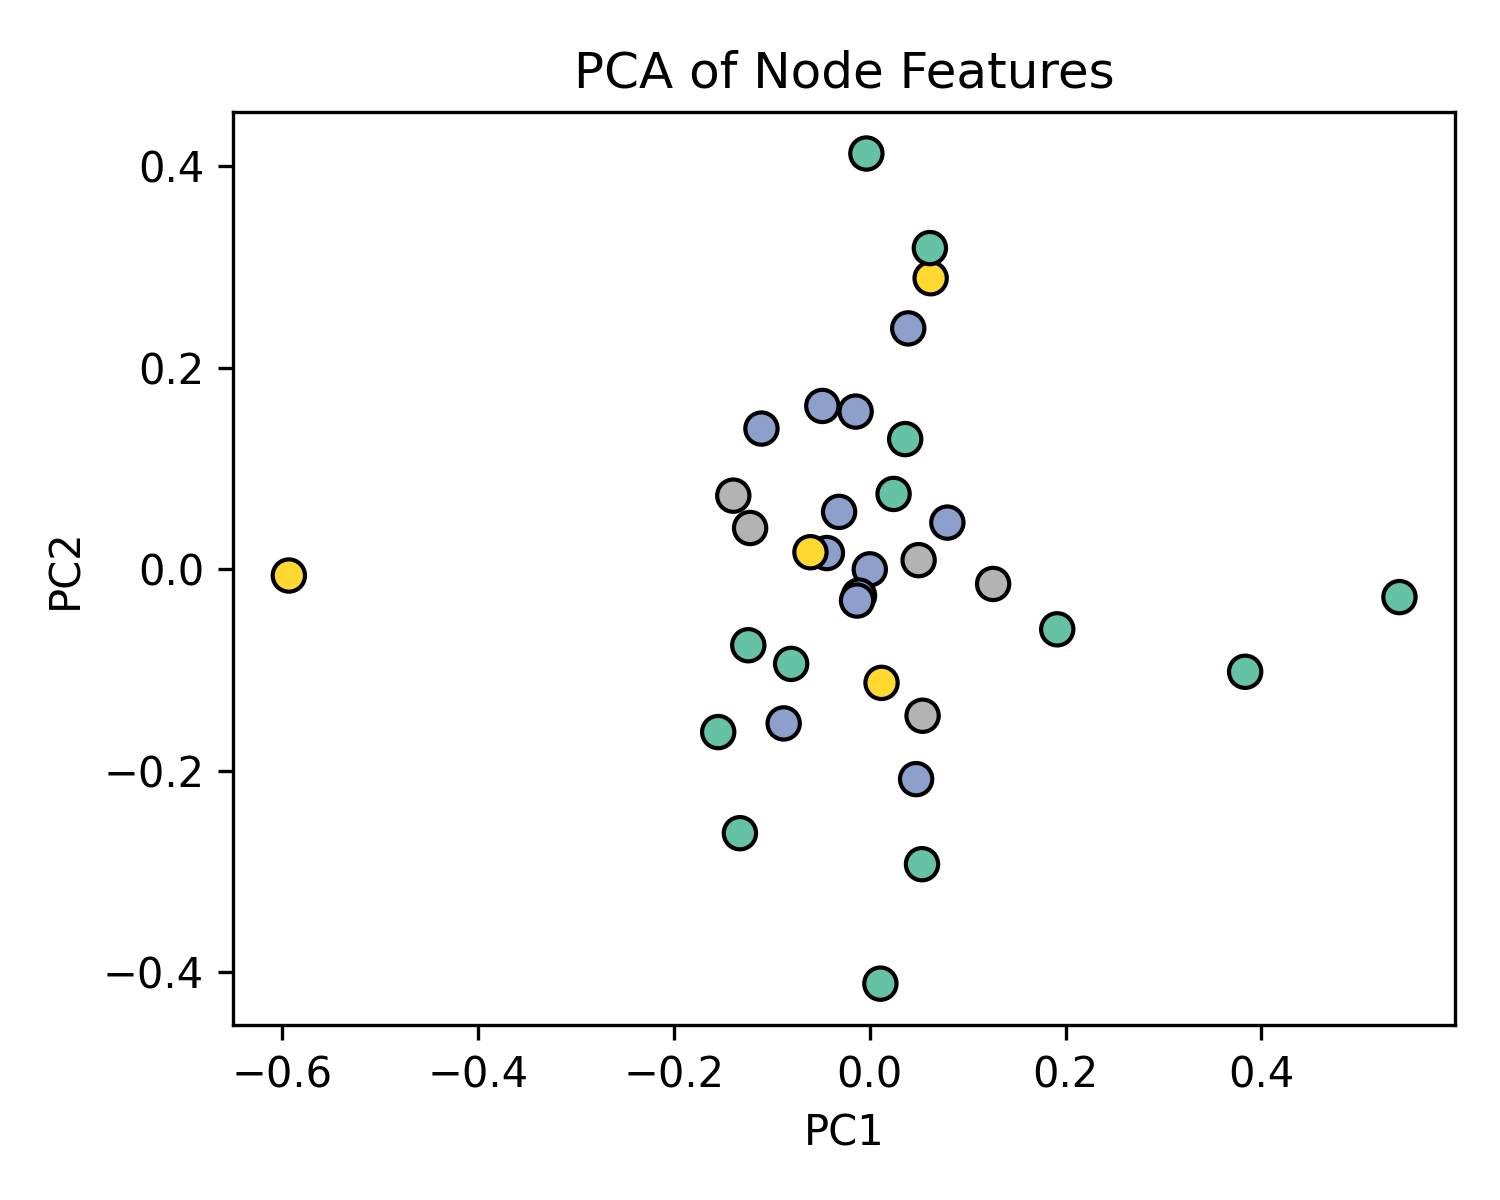
\includegraphics[width=0.75\linewidth]{node_features_pca.png}
    \caption{PCA of node features; colors indicate the node labels.}
    \label{fig:node_feat_pca}
\end{figure}

\section{Part E: Combining structure and node features}
We concatenate the structural features from Part~C with the node features to form $X_{\text{comb}} = [X_{\text{struct}} \; X_{\text{attr}}]$. We train the same two classifiers (MLP and logistic regression) on $X_{\text{comb}}$ and evaluate them with stratified 5-fold cross-validation (seed 42). The mean test accuracies are:
\begin{itemize}
    \item \textbf{MLP:} \textbf{38.10\%} $\pm$ \textbf{14.13\%} (mean train accuracy 100\%).
    \item \textbf{Logistic Regression:} \textbf{40.95\%} $\pm$ \textbf{13.33\%} (mean train accuracy 100\%).
\end{itemize}
The implementation is shown in Listing~\ref{lst:e1}.

\section{Part F: Cora node classification (Planetoid)}
We repeat the node label prediction on the Cora dataset using the official PyG masks (\texttt{train\_mask}, \texttt{val\_mask}, \texttt{test\_mask}). We use the same structural features as in Part~C (6 structural statistics), the raw node features $X_{\text{attr}}=\texttt{data.x}$, and their concatenation $X_{\text{comb}}=[X_{\text{struct}} \; X_{\text{attr}}]$. A small MLP (input $\rightarrow$ 64 $\rightarrow$ 7) with ReLU and dropout is trained with Adam (lr=0.01, weight decay $5\times10^{-4}$) and early stopping on validation accuracy. The best validation and corresponding test accuracies are:

\begin{table}[H]
    \centering
    \begin{tabular}{lcc}
        \hline
        Input features & Val acc & Test acc \\
        \hline
        $X_{\text{struct}}$ & 27.0\% & 27.7\% \\
        $X_{\text{attr}}$ & 61.2\% & 57.3\% \\
        $X_{\text{comb}}$ & 59.2\% & 56.9\% \\
        \hline
    \end{tabular}
    \caption{Cora node classification using official Planetoid splits.}
    \label{tab:cora_results}
\end{table}
The implementation is shown in Listing~\ref{lst:f1}.

\section{Part G: Short discussion}
\begin{enumerate}
    \item \textbf{Best input.} On Cora, node features ($X_{\text{attr}}$) performed best (highest validation and test accuracy). Structural features alone were the weakest.
    \item \textbf{Why combining helps or not.} Combining did not help here because the structural features are relatively coarse and less aligned with topic labels than the bag-of-words node features. Concatenating them can add noise and increase dimensionality without adding strong predictive signal, which can slightly hurt or leave performance unchanged unless the model and hyperparameters are tuned for the mix.
    \item \textbf{What structure captures.} Structural features capture graph-topology information such as degree, centrality, clustering, and neighborhood connectivity patterns, i.e., how a node is positioned in the citation network. This relational role information is not present in the raw node attributes.
\end{enumerate}

\section{2. Node2Vec vs Struct2Vec on GeometricShapes}
\subsection{Part A: Load graphs and visualize the original geometry}
We load the GeometricShapes dataset with \texttt{FaceToEdge} to populate \texttt{edge\_index}, select three graphs (indices 0, 1, 2), and plot their original geometry using \texttt{data.pos} with edges drawn from \texttt{data.edge\_index}.
\begin{figure}[H]
    \centering
    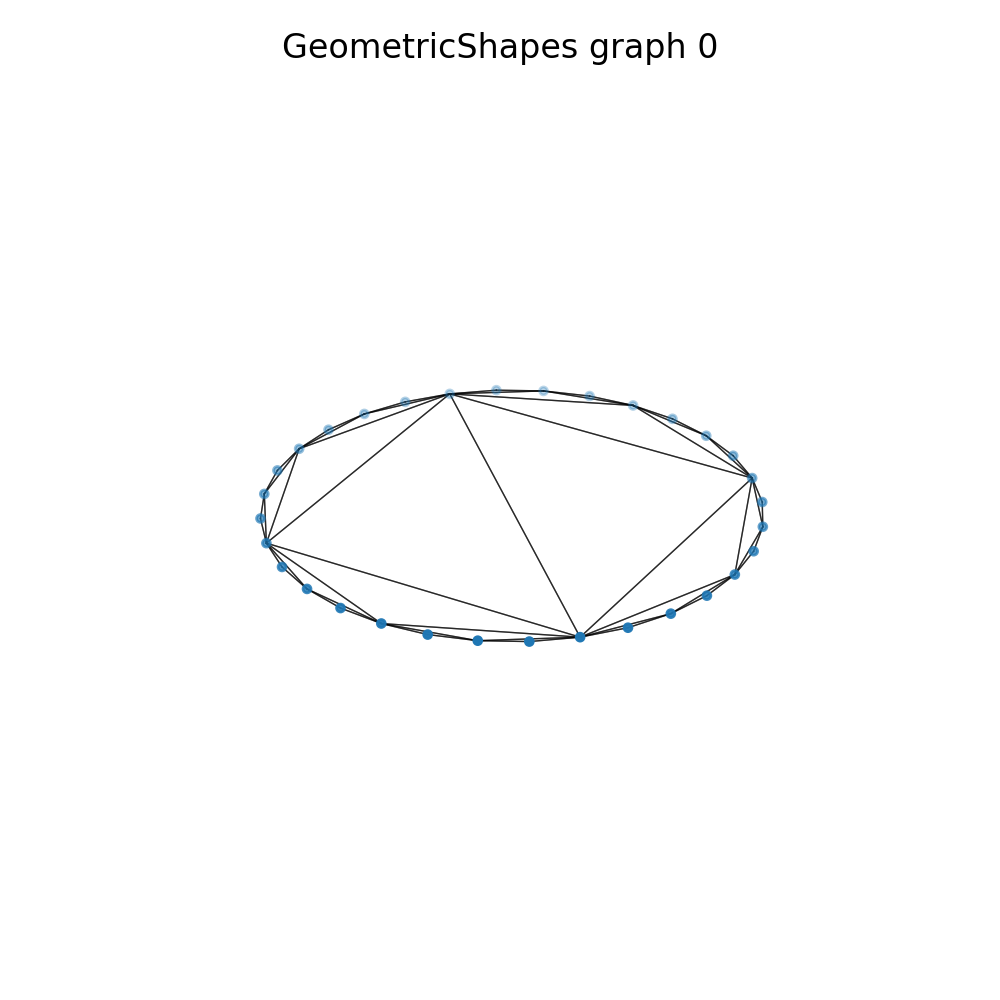
\includegraphics[width=0.32\linewidth]{geometric_shapes_graph0.png}
    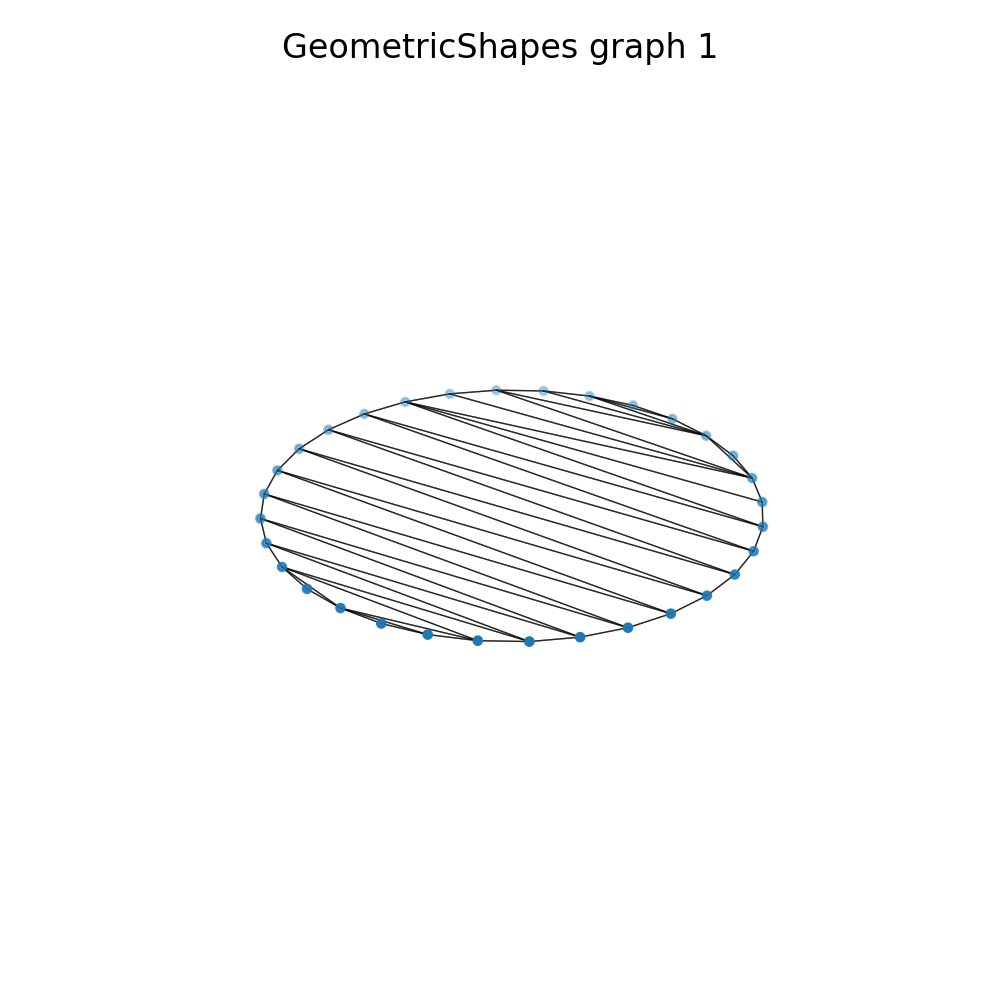
\includegraphics[width=0.32\linewidth]{geometric_shapes_graph1.png}
    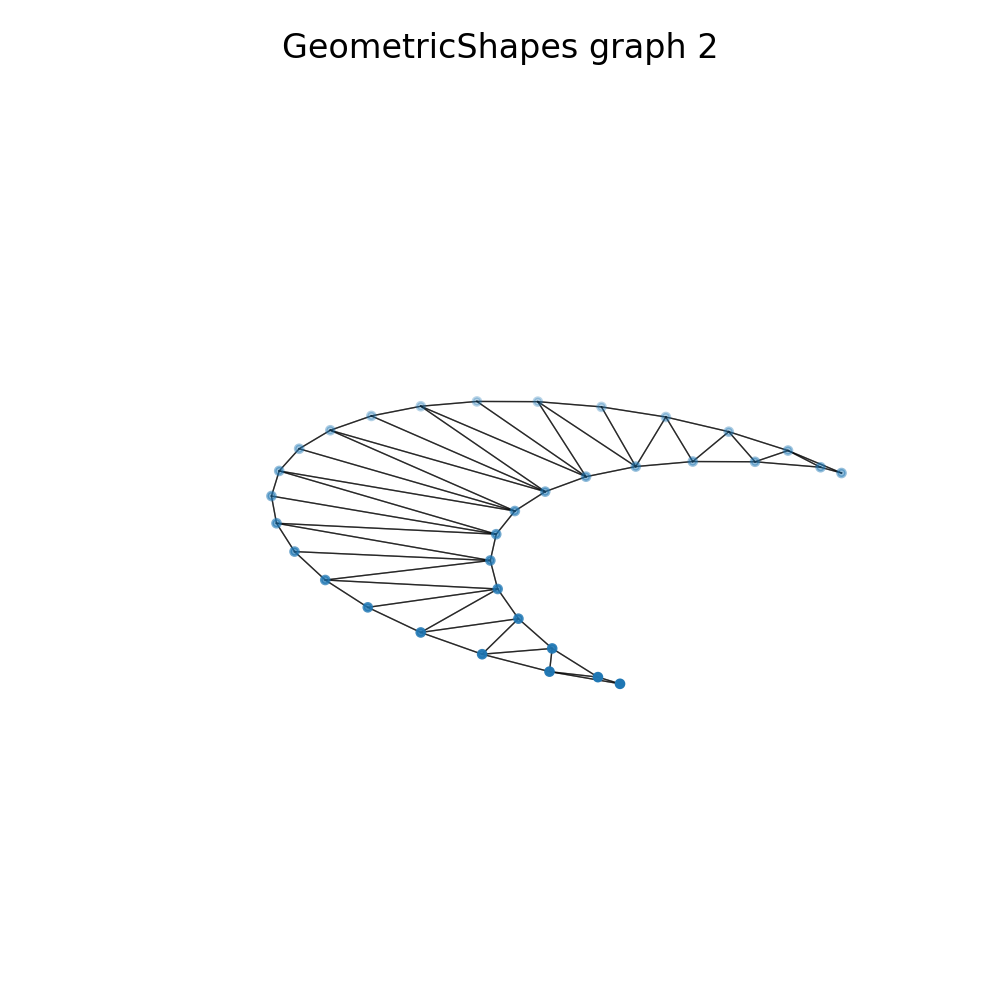
\includegraphics[width=0.32\linewidth]{geometric_shapes_graph2.png}
    \caption{Original geometry for GeometricShapes graphs 0, 1, and 2 (left to right).}
\end{figure}

\subsection{Part B: Node2Vec embeddings and visualization}
\subsubsection{B1. Implement biased random walks}
We implement the Node2Vec transition rule on an undirected graph and use $p=10$. For BFS-like and DFS-like behavior, we vary $q$ and report both values in the results.
\subsubsection{B2. Generate training walks}
For each node, we generate multiple walks with a fixed length of 20 (10 walks per node in our runs) to build the skip-gram training corpus.
\subsubsection{B3. Learn embeddings}
We train a skip-gram model with negative sampling to produce 2D embeddings ($d=2$). We run Node2Vec with two settings: BFS-like walks ($q=0.5$) and DFS-like walks ($q=5$), then plot the graph using the learned embedding coordinates and the same edges.
\begin{figure}[H]
    \centering
    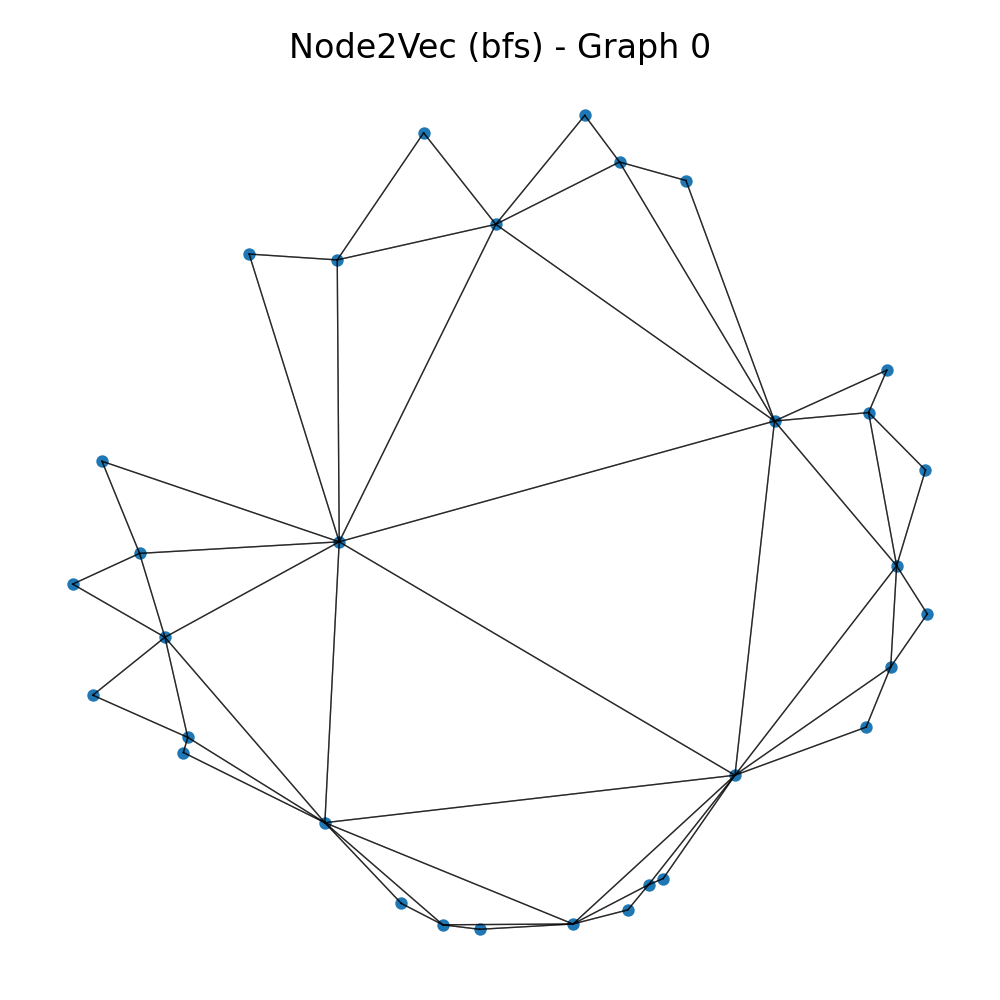
\includegraphics[width=0.49\linewidth]{node2vec_graph0_bfs.png}
    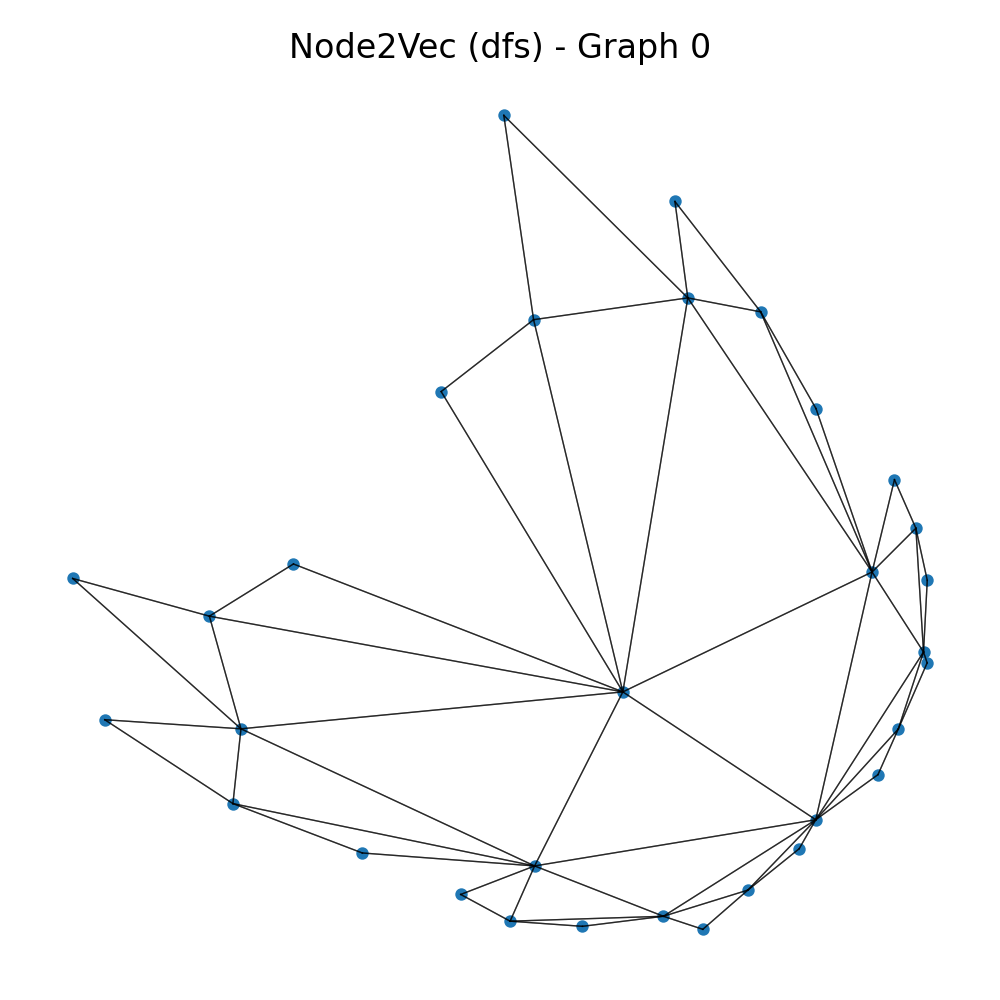
\includegraphics[width=0.49\linewidth]{node2vec_graph0_dfs.png}
    \caption{Node2Vec embeddings for graph 0 (left: BFS-like, right: DFS-like).}
\end{figure}
\begin{figure}[H]
    \centering
    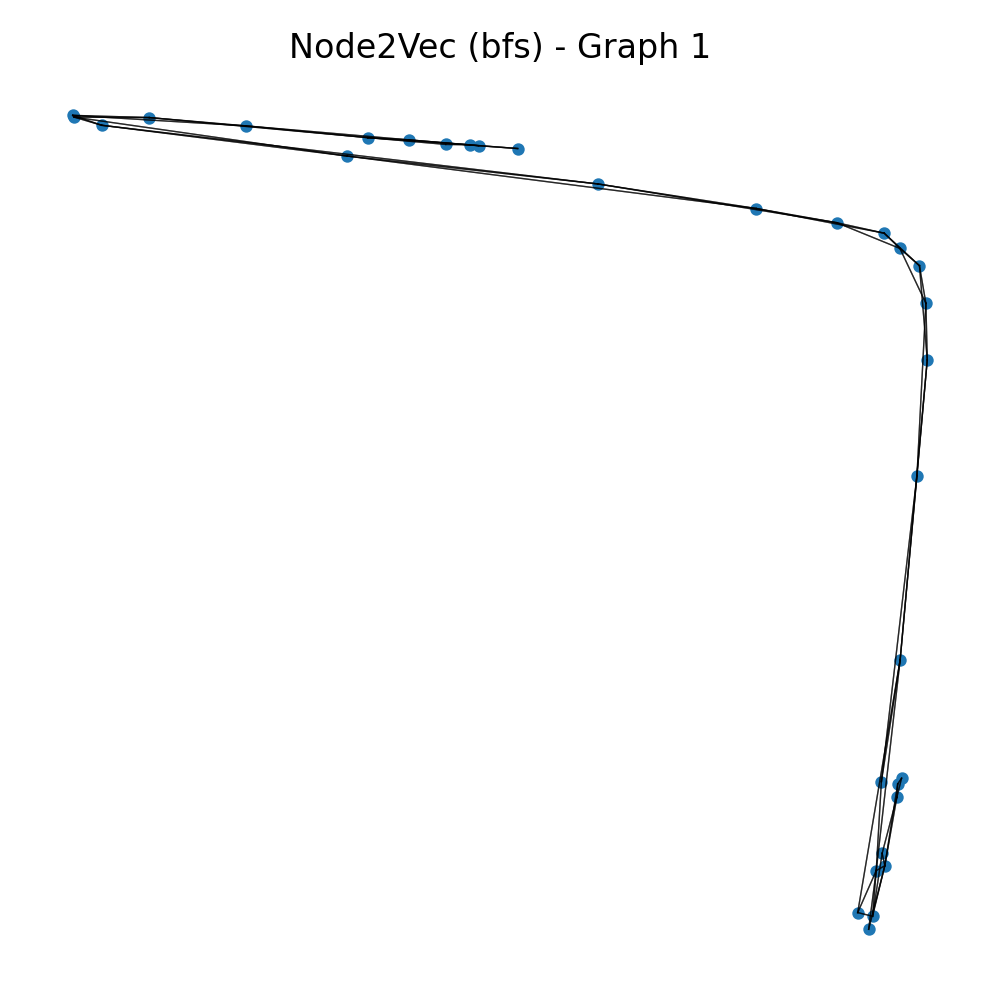
\includegraphics[width=0.49\linewidth]{node2vec_graph1_bfs.png}
    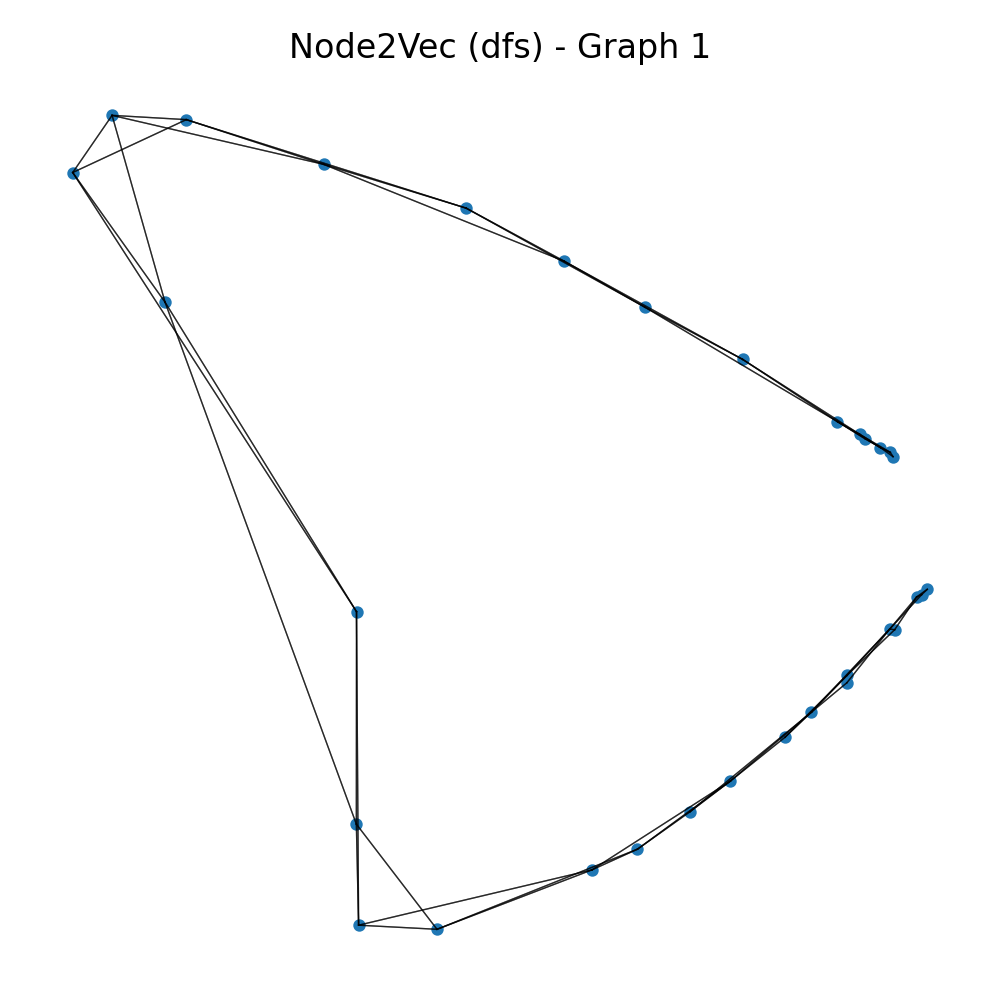
\includegraphics[width=0.49\linewidth]{node2vec_graph1_dfs.png}
    \caption{Node2Vec embeddings for graph 1 (left: BFS-like, right: DFS-like).}
\end{figure}
\begin{figure}[H]
    \centering
    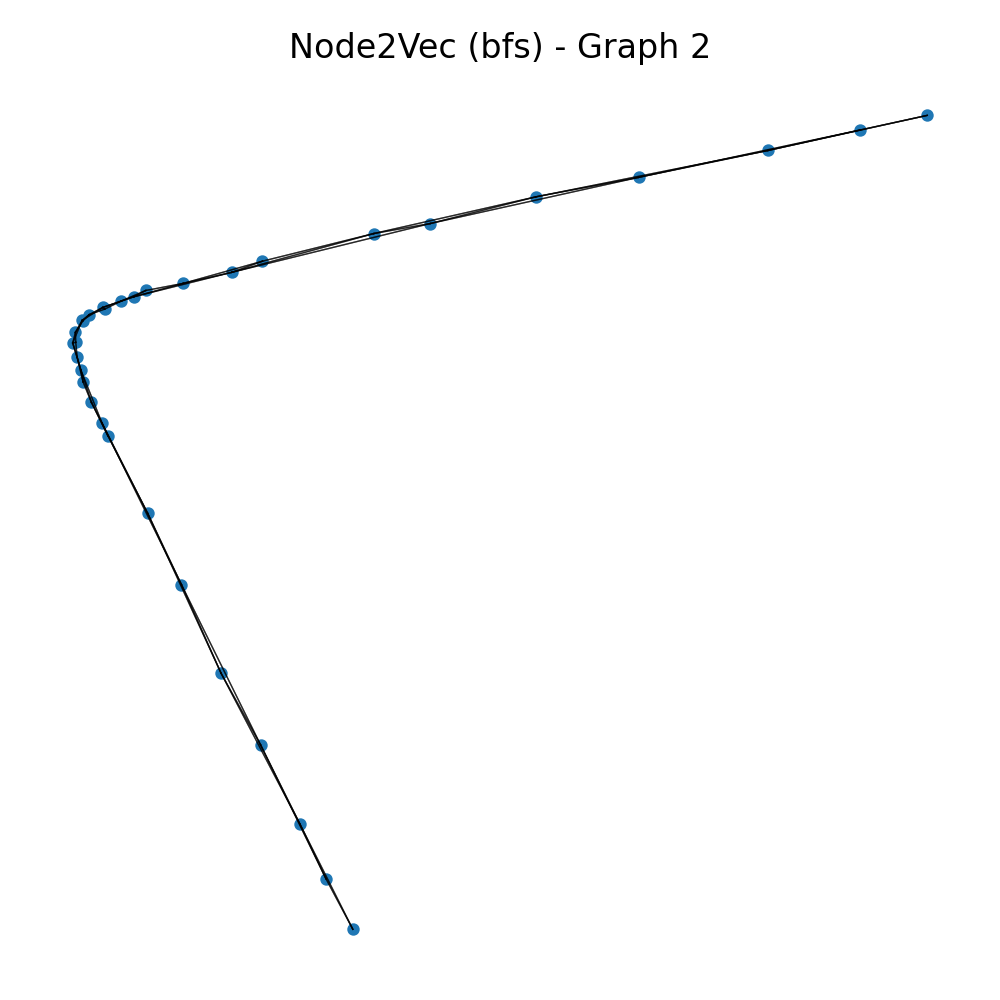
\includegraphics[width=0.49\linewidth]{node2vec_graph2_bfs.png}
    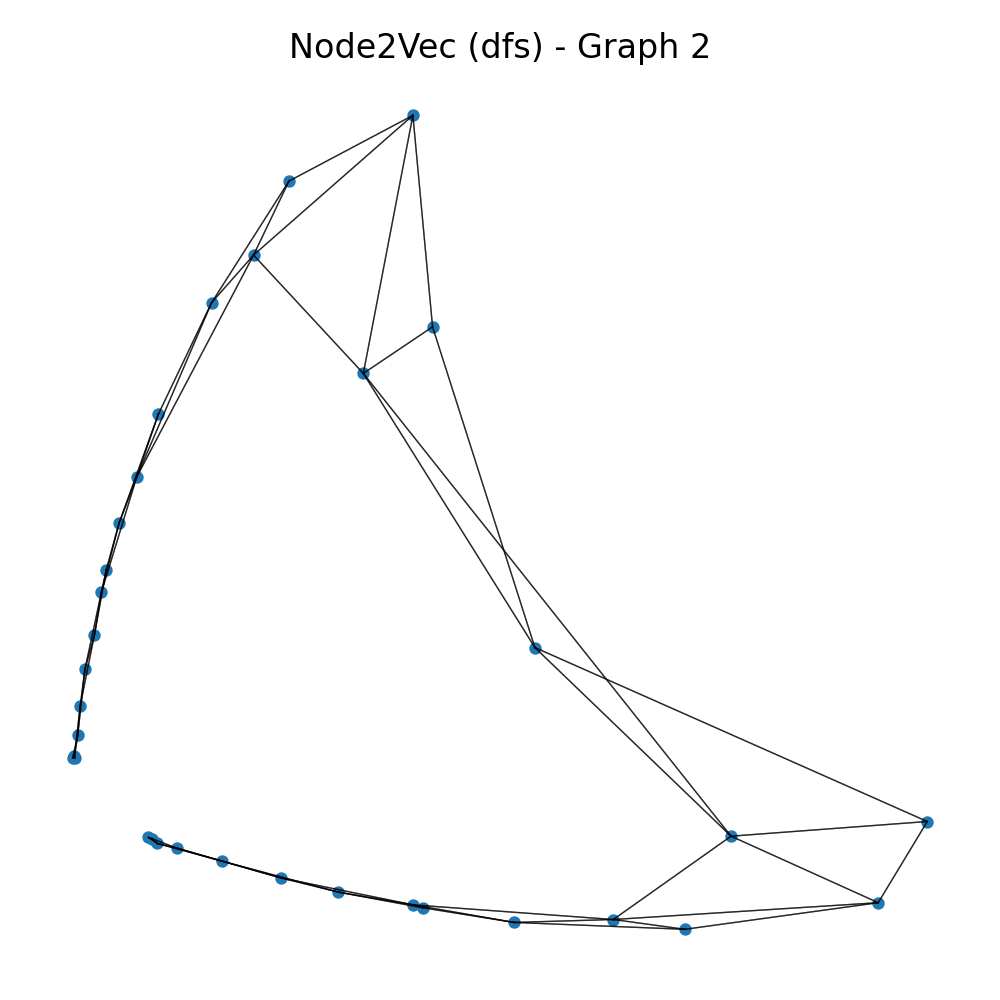
\includegraphics[width=0.49\linewidth]{node2vec_graph2_dfs.png}
    \caption{Node2Vec embeddings for graph 2 (left: BFS-like, right: DFS-like).}
\end{figure}

\subsection{Part C: Struct2Vec embeddings and visualization (fixed k=3)}
\subsubsection{C1. Structural similarity function $g_k(u,v)$}
\subsubsection{C2. Construct the Struct2Vec graph}
\subsubsection{C3. Random walks on the Struct2Vec graph}
\subsubsection{C4. Learn embeddings}

\subsection{Part D: Comparison questions (short answers)}

\section{3. Graph-Based Sentiment Analysis with Node2Vec}
\subsection{Part A: Construct a word co-occurrence graph}
\subsubsection{A1. Text preprocessing}
\subsubsection{A2. Build the word graph}

\subsection{Part B: Learn word embeddings using Node2Vec}
\subsubsection{B1. Apply Node2Vec}
\subsubsection{B2. Inspect embeddings}

\subsection{Part C: Text representation using graph embeddings}
\subsubsection{C1. Document embeddings}

\subsection{Part D: Sentiment classification}
\subsubsection{D1. Train a classifier}

\subsection{Part E: Short discussion}
\appendix
\section{Code}
\begin{lstlisting}[language=Python,caption={Part A code}]
from torch_geometric.datasets import KarateClub

dataset = KarateClub()
data = dataset[0]
print(f"Number of nodes: {data.num_nodes}")
print(f"Number of edges: {data.num_edges}")
if data.x is not None:
    print(f"data.x shape: {data.x.shape}")
else:
    print("data.x shape: None")
print(f"data.edge_index shape: {data.edge_index.shape}")
print(f"Number of node labels/classes: {dataset.num_classes}")
\end{lstlisting}

\section{Graph Visualization Code}
\begin{lstlisting}[language=Python,caption={Part A graph visualization}]
import matplotlib
matplotlib.use("Agg")
import matplotlib.pyplot as plt
import networkx as nx
from torch_geometric.datasets import KarateClub
from torch_geometric.utils import to_networkx

dataset = KarateClub()
data = dataset[0]

# Convert PyG graph to NetworkX
G = to_networkx(data, to_undirected=True)

# Node colors based on labels
labels = data.y.tolist()

# Define colors to match the figure legend
color_map = {
    0: "#66C2A5",
    1: "#FC8D62",
    2: "#8DA0CB",
    3: "#FFD92F",
}
node_colors = [color_map[label] for label in labels]

# Draw the graph
pos = nx.spring_layout(G, seed=42)
plt.figure(figsize=(6, 5))
nx.draw(
    G,
    pos,
    node_color=node_colors,
    with_labels=True,
    node_size=400,
    font_size=8,
)
plt.title("Karate Club Graph")
plt.tight_layout()
plt.savefig("karate_club_graph.png", dpi=300)
\end{lstlisting}

\section{GeometricShapes Visualization Code}
\begin{lstlisting}[language=Python,caption={GeometricShapes visualization (Part 2A)}]
import matplotlib
matplotlib.use("Agg")
import matplotlib.pyplot as plt
import numpy as np
from torch_geometric.datasets import GeometricShapes
from torch_geometric.transforms import FaceToEdge


def plot_graph(data, idx):
    pos = data.pos.cpu().numpy()
    edge_index = data.edge_index.cpu().numpy()
    dim = pos.shape[1]

    fig = plt.figure(figsize=(5, 5))
    if dim == 3:
        ax = fig.add_subplot(111, projection="3d")
        ax.scatter(pos[:, 0], pos[:, 1], pos[:, 2], s=8, c="tab:blue")
        for u, v in edge_index.T:
            xs = [pos[u, 0], pos[v, 0]]
            ys = [pos[u, 1], pos[v, 1]]
            zs = [pos[u, 2], pos[v, 2]]
            ax.plot(xs, ys, zs, color="black", linewidth=0.5, alpha=0.6)
    else:
        ax = fig.add_subplot(111)
        ax.scatter(pos[:, 0], pos[:, 1], s=8, c="tab:blue")
        for u, v in edge_index.T:
            xs = [pos[u, 0], pos[v, 0]]
            ys = [pos[u, 1], pos[v, 1]]
            ax.plot(xs, ys, color="black", linewidth=0.5, alpha=0.6)
        ax.set_aspect("equal", adjustable="box")

    ax.set_title(f"GeometricShapes graph {idx}")
    ax.axis("off")
    return fig


# Load dataset with FaceToEdge so edge_index is populated
transform = FaceToEdge()

dataset = GeometricShapes(root="data/GeometricShapes", pre_transform=transform)

# Pick any 3 graphs
indices = [0, 1, 2]
for idx in indices:
    fig = plot_graph(dataset[idx], idx)
    fig.tight_layout()
    fig.savefig(f"geometric_shapes_graph{idx}.png", dpi=200)
    plt.close(fig)
\end{lstlisting}

\section{Node2Vec (Biased Walks + Skip-gram) Code}
\begin{lstlisting}[language=Python,caption={Node2Vec on GeometricShapes (Part 2B)}]
import math
import numpy as np
import torch
import torch.nn.functional as F
from torch import nn, optim
import matplotlib
matplotlib.use("Agg")
import matplotlib.pyplot as plt
from torch_geometric.datasets import GeometricShapes
from torch_geometric.transforms import FaceToEdge


def build_undirected_adj(num_nodes, edge_index):
    adj = [set() for _ in range(num_nodes)]
    src, dst = edge_index
    for u, v in zip(src, dst):
        u = int(u)
        v = int(v)
        adj[u].add(v)
        adj[v].add(u)
    return adj


def node2vec_walk(start, walk_length, adj, p, q, rng):
    walk = [start]
    while len(walk) < walk_length:
        v = walk[-1]
        neighbors = list(adj[v])
        if not neighbors:
            break
        if len(walk) == 1:
            next_node = rng.choice(neighbors)
        else:
            t = walk[-2]
            weights = []
            t_neighbors = adj[t]
            for x in neighbors:
                if x == t:
                    w = 1.0 / p
                elif x in t_neighbors:
                    w = 1.0
                else:
                    w = 1.0 / q
                weights.append(w)
            weights = np.asarray(weights, dtype=np.float64)
            probs = weights / weights.sum()
            next_node = rng.choice(neighbors, p=probs)
        walk.append(int(next_node))
    return walk


def generate_walks(adj, num_walks_per_node, walk_length, p, q, seed=42):
    rng = np.random.default_rng(seed)
    walks = []
    nodes = list(range(len(adj)))
    for _ in range(num_walks_per_node):
        rng.shuffle(nodes)
        for start in nodes:
            walks.append(node2vec_walk(start, walk_length, adj, p, q, rng))
    return walks


def build_pairs(walks, window_size):
    pairs = []
    for walk in walks:
        for i, center in enumerate(walk):
            left = max(0, i - window_size)
            right = min(len(walk), i + window_size + 1)
            for j in range(left, right):
                if i == j:
                    continue
                pairs.append((center, walk[j]))
    return pairs


def build_negative_sampling_dist(walks, num_nodes, power=0.75):
    counts = np.zeros(num_nodes, dtype=np.float64)
    for walk in walks:
        for node in walk:
            counts[node] += 1
    counts = np.power(counts, power)
    counts[counts == 0] = 1.0
    probs = counts / counts.sum()
    return torch.tensor(probs, dtype=torch.float32)


def train_skipgram(
    num_nodes,
    pairs,
    neg_dist,
    embedding_dim=2,
    num_negatives=5,
    epochs=50,
    batch_size=256,
    lr=0.01,
    seed=42,
):
    torch.manual_seed(seed)
    device = torch.device("cpu")

    emb_in = nn.Embedding(num_nodes, embedding_dim).to(device)
    emb_out = nn.Embedding(num_nodes, embedding_dim).to(device)
    optimizer = optim.Adam(list(emb_in.parameters()) + list(emb_out.parameters()), lr=lr)

    pairs = np.asarray(pairs, dtype=np.int64)
    num_pairs = len(pairs)

    for epoch in range(epochs):
        perm = np.random.permutation(num_pairs)
        for start in range(0, num_pairs, batch_size):
            idx = perm[start : start + batch_size]
            batch = pairs[idx]
            centers = torch.tensor(batch[:, 0], dtype=torch.long, device=device)
            contexts = torch.tensor(batch[:, 1], dtype=torch.long, device=device)

            center_vecs = emb_in(centers)
            context_vecs = emb_out(contexts)
            pos_scores = torch.sum(center_vecs * context_vecs, dim=1)
            pos_loss = -F.logsigmoid(pos_scores).mean()

            neg_samples = torch.multinomial(
                neg_dist, centers.size(0) * num_negatives, replacement=True
            ).to(device)
            neg_samples = neg_samples.view(centers.size(0), num_negatives)
            neg_vecs = emb_out(neg_samples)
            neg_scores = torch.sum(center_vecs.unsqueeze(1) * neg_vecs, dim=2)
            neg_loss = -F.logsigmoid(-neg_scores).mean()

            loss = pos_loss + neg_loss
            optimizer.zero_grad()
            loss.backward()
            optimizer.step()

    return emb_in.weight.detach().cpu().numpy()


def plot_embedding(data, emb, title, out_path):
    edge_index = data.edge_index.cpu().numpy()
    fig, ax = plt.subplots(figsize=(5, 5))
    for u, v in edge_index.T:
        xs = [emb[u, 0], emb[v, 0]]
        ys = [emb[u, 1], emb[v, 1]]
        ax.plot(xs, ys, color="black", linewidth=0.5, alpha=0.6)
    ax.scatter(emb[:, 0], emb[:, 1], s=12, c="tab:blue")
    ax.set_title(title)
    ax.axis("off")
    fig.tight_layout()
    fig.savefig(out_path, dpi=200)
    plt.close(fig)


if __name__ == "__main__":
    # Node2Vec parameters (reported in the writeup)
    p = 10
    q_bfs = 0.5
    q_dfs = 5
    print(f"Node2Vec parameters: p={p}, q_bfs={q_bfs}, q_dfs={q_dfs}")

    dataset = GeometricShapes(root="data/GeometricShapes", pre_transform=FaceToEdge())
    indices = [0, 1, 2]

    for idx in indices:
        data = dataset[idx]
        adj = build_undirected_adj(data.num_nodes, data.edge_index)
        for label, q in [("bfs", q_bfs), ("dfs", q_dfs)]:
            walks = generate_walks(
                adj,
                num_walks_per_node=10,
                walk_length=20,
                p=p,
                q=q,
                seed=42,
            )
            pairs = build_pairs(walks, window_size=5)
            neg_dist = build_negative_sampling_dist(walks, data.num_nodes)
            emb = train_skipgram(
                data.num_nodes,
                pairs,
                neg_dist,
                embedding_dim=2,
                num_negatives=5,
                epochs=50,
                batch_size=256,
                lr=0.01,
                seed=42,
            )
            out_path = f"node2vec_graph{idx}_{label}.png"
            title = f"Node2Vec ({label}) - Graph {idx}"
            plot_embedding(data, emb, title, out_path)
            print(
                f"Graph {idx} [{label}]: walks={len(walks)}, pairs={len(pairs)}, saved {out_path}"
            )
\end{lstlisting}

\section{Structural Features Code}
\begin{lstlisting}[language=Python,caption={Part C1 structural features}]
import math
from torch_geometric.datasets import KarateClub


def build_undirected_adj(num_nodes, edge_index):
    adj = [set() for _ in range(num_nodes)]
    for u, v in zip(edge_index[0], edge_index[1]):
        u = int(u)
        v = int(v)
        if u == v:
            continue
        adj[u].add(v)
        adj[v].add(u)
    return adj


def bfs_distances(adj, source):
    n = len(adj)
    dist = [-1] * n
    dist[source] = 0
    queue = [source]
    head = 0
    while head < len(queue):
        u = queue[head]
        head += 1
        for v in adj[u]:
            if dist[v] == -1:
                dist[v] = dist[u] + 1
                queue.append(v)
    return dist


def betweenness_centrality(adj):
    n = len(adj)
    bc = [0.0] * n
    for s in range(n):
        stack = []
        pred = [[] for _ in range(n)]
        sigma = [0.0] * n
        dist = [-1] * n
        sigma[s] = 1.0
        dist[s] = 0
        queue = [s]
        head = 0
        while head < len(queue):
            v = queue[head]
            head += 1
            stack.append(v)
            for w in adj[v]:
                if dist[w] < 0:
                    dist[w] = dist[v] + 1
                    queue.append(w)
                if dist[w] == dist[v] + 1:
                    sigma[w] += sigma[v]
                    pred[w].append(v)
        delta = [0.0] * n
        while stack:
            w = stack.pop()
            for v in pred[w]:
                if sigma[w] != 0:
                    delta[v] += (sigma[v] / sigma[w]) * (1.0 + delta[w])
            if w != s:
                bc[w] += delta[w]
    for i in range(n):
        bc[i] /= 2.0
    if n > 2:
        scale = 1.0 / ((n - 1) * (n - 2) / 2.0)
        bc = [x * scale for x in bc]
    return bc


def closeness_centrality(adj):
    n = len(adj)
    cc = [0.0] * n
    for u in range(n):
        dist = bfs_distances(adj, u)
        total = 0
        reachable = 0
        for d in dist:
            if d > 0:
                total += d
                reachable += 1
        if total > 0 and reachable > 0:
            cc[u] = reachable / total
    return cc


def pagerank(adj, damping=0.85, max_iter=100, tol=1e-6):
    n = len(adj)
    pr = [1.0 / n] * n
    out_deg = [len(adj[u]) for u in range(n)]
    for _ in range(max_iter):
        new_pr = [(1.0 - damping) / n] * n
        for u in range(n):
            if out_deg[u] == 0:
                share = damping * pr[u] / n
                for v in range(n):
                    new_pr[v] += share
            else:
                share = damping * pr[u] / out_deg[u]
                for v in adj[u]:
                    new_pr[v] += share
        diff = 0.0
        for i in range(n):
            diff += abs(new_pr[i] - pr[i])
        pr = new_pr
        if diff < tol:
            break
    return pr


def eigenvector_centrality(adj, max_iter=100, tol=1e-6):
    n = len(adj)
    x = [1.0] * n
    for _ in range(max_iter):
        x_new = [0.0] * n
        for u in range(n):
            for v in adj[u]:
                x_new[u] += x[v]
        norm = math.sqrt(sum(val * val for val in x_new))
        if norm == 0:
            break
        x_new = [val / norm for val in x_new]
        diff = sum(abs(x_new[i] - x[i]) for i in range(n))
        x = x_new
        if diff < tol:
            break
    return x


def clustering_coefficient(adj):
    n = len(adj)
    cc = [0.0] * n
    for u in range(n):
        neighbors = list(adj[u])
        k = len(neighbors)
        if k < 2:
            cc[u] = 0.0
            continue
        links = 0
        for i in range(k):
            for j in range(i + 1, k):
                if neighbors[j] in adj[neighbors[i]]:
                    links += 1
        cc[u] = (2.0 * links) / (k * (k - 1))
    return cc


def zscore_columns(matrix):
    n = len(matrix)
    m = len(matrix[0])
    means = [0.0] * m
    stds = [0.0] * m
    for j in range(m):
        s = 0.0
        for i in range(n):
            s += matrix[i][j]
        means[j] = s / n
    for j in range(m):
        s = 0.0
        for i in range(n):
            diff = matrix[i][j] - means[j]
            s += diff * diff
        stds[j] = math.sqrt(s / n)
        if stds[j] == 0:
            stds[j] = 1.0
    for i in range(n):
        for j in range(m):
            matrix[i][j] = (matrix[i][j] - means[j]) / stds[j]
    return matrix


def compute_structural_features(adj, node_order=None, normalize=True):
    """
    Compute structural features for each node and stack them into a matrix.
    Features: degree, betweenness, closeness, PageRank, eigenvector, clustering.
    """
    n = len(adj)
    if node_order is None:
        node_order = list(range(n))

    degree = [len(adj[u]) for u in range(n)]
    betweenness = betweenness_centrality(adj)
    closeness = closeness_centrality(adj)
    pr = pagerank(adj)
    eigen = eigenvector_centrality(adj)
    cluster = clustering_coefficient(adj)

    X = []
    for node in node_order:
        X.append(
            [
                degree[node],
                betweenness[node],
                closeness[node],
                pr[node],
                eigen[node],
                cluster[node],
            ]
        )

    if normalize:
        X = zscore_columns(X)

    return X


def main():
    dataset = KarateClub()
    data = dataset[0]

    adj = build_undirected_adj(data.num_nodes, data.edge_index)
    node_order = list(range(data.num_nodes))
    X_struct = compute_structural_features(adj, node_order=node_order, normalize=True)

    print("Structural embedding matrix shape:", (len(X_struct), len(X_struct[0])))
    print("First 5 rows:")
    for row in X_struct[:5]:
        print(row)


if __name__ == "__main__":
    main()
\end{lstlisting}

\section{Structural Embeddings Visualization Code}
\begin{lstlisting}[language=Python,caption={Part C2 PCA visualization}]
import numpy as np
import matplotlib
matplotlib.use("Agg")
import matplotlib.pyplot as plt
import matplotlib.colors as mcolors
from torch_geometric.datasets import KarateClub

from structural_features import build_undirected_adj, compute_structural_features


def pca_2d(features):
    X = np.array(features, dtype=float)
    X_centered = X - X.mean(axis=0, keepdims=True)
    cov = np.cov(X_centered, rowvar=False)
    eigvals, eigvecs = np.linalg.eigh(cov)
    order = np.argsort(eigvals)[::-1]
    eigvals_sorted = eigvals[order]
    eigvecs_sorted = eigvecs[:, order]
    components = eigvecs_sorted[:, :2]
    emb_2d = X_centered @ components
    return emb_2d, components, eigvals_sorted


def main():
    dataset = KarateClub()
    data = dataset[0]

    adj = build_undirected_adj(data.num_nodes, data.edge_index)
    node_order = list(range(data.num_nodes))

    X_struct = compute_structural_features(
        adj,
        node_order=node_order,
        should_normalize=True,
    )
    emb_2d, components, eigvals_sorted = pca_2d(X_struct)

    feature_names = [
        "degree",
        "betweenness",
        "closeness",
        "pagerank",
        "eigenvector",
        "clustering",
    ]

    if components.shape[0] != len(feature_names):
        print(
            f"[WARN] components has {components.shape[0]} rows (features), but feature_names has {len(feature_names)}. "
            "Update feature_names to match compute_structural_features column order/length."
        )

    total_var = float(np.sum(eigvals_sorted)) if np.sum(eigvals_sorted) != 0 else 1.0
    evr = eigvals_sorted / total_var
    print("\nExplained variance ratio:")
    print(f"  PC1: {evr[0]:.4f}")
    print(f"  PC2: {evr[1]:.4f}")

    for pc_idx in range(2):
        pc_name = f"PC{pc_idx + 1}"
        print(f"\n{pc_name} loadings (feature weights):")

        pairs = []
        for i in range(min(len(feature_names), components.shape[0])):
            pairs.append((feature_names[i], float(components[i, pc_idx])))

        pairs.sort(key=lambda x: abs(x[1]), reverse=True)

        for fname, w in pairs:
            print(f"  {fname:12s} {w:+.6f}")

    labels = data.y.tolist()
    classes = sorted(set(int(v) for v in labels))
    class_to_idx = {c: i for i, c in enumerate(classes)}
    labels_idx = np.array([class_to_idx[int(v)] for v in labels], dtype=int)

    cmap = plt.cm.get_cmap("Set2", len(classes))
    bounds = np.arange(-0.5, len(classes) + 0.5, 1)
    norm = mcolors.BoundaryNorm(bounds, cmap.N)

    plt.figure(figsize=(6, 5))
    scatter = plt.scatter(
        emb_2d[:, 0],
        emb_2d[:, 1],
        c=labels_idx,
        cmap=cmap,
        norm=norm,
        s=70,
        edgecolors="k",
        linewidths=0.4,
    )
    plt.title("PCA of Structural Features")
    plt.xlabel("PC1")
    plt.ylabel("PC2")

    cbar = plt.colorbar(scatter, ticks=np.arange(len(classes)))
    cbar.set_ticklabels([str(c) for c in classes])
    cbar.set_label("data.y class")

    plt.tight_layout()
    plt.savefig("structural_pca.png", dpi=200)
    plt.close()


if __name__ == "__main__":
    main()
\end{lstlisting}

\section{Node Classification Code}
\begin{lstlisting}[language=Python,caption={Part C3 node classification using structural features},label={lst:c3}]
import random
import numpy as np
import torch
from torch import nn
from torch_geometric.datasets import KarateClub
from sklearn.model_selection import StratifiedKFold

from structural_features import build_undirected_adj, compute_structural_features


def set_seed(seed: int) -> None:
    random.seed(seed)
    np.random.seed(seed)
    torch.manual_seed(seed)


def build_mlp(input_dim, num_classes):
    return nn.Sequential(
        nn.Linear(input_dim, 16),
        nn.ReLU(),
        nn.Linear(16, num_classes),
    )


def build_logreg(input_dim, num_classes):
    return nn.Linear(input_dim, num_classes)


def train_classifier(model, x, y, train_idx, epochs=500, lr=0.05, weight_decay=1e-4):
    optimizer = torch.optim.Adam(model.parameters(), lr=lr, weight_decay=weight_decay)
    criterion = nn.CrossEntropyLoss()

    for _ in range(epochs):
        model.train()
        logits = model(x)
        loss = criterion(logits[train_idx], y[train_idx])
        optimizer.zero_grad()
        loss.backward()
        optimizer.step()

    return model


def accuracy(model, x, y, idx):
    model.eval()
    with torch.no_grad():
        preds = model(x).argmax(dim=1)
        correct = (preds[idx] == y[idx]).sum().item()
        total = idx.numel()
    return correct / total if total > 0 else 0.0


def main():
    set_seed(42)

    dataset = KarateClub()
    data = dataset[0]

    adj = build_undirected_adj(data.num_nodes, data.edge_index)
    node_order = list(range(data.num_nodes))
    x_struct = compute_structural_features(
        adj,
        node_order=node_order,
        should_normalize=True,
    )

    x = torch.tensor(x_struct, dtype=torch.float32)
    y = data.y.clone().long()

    num_classes = dataset.num_classes

    skf = StratifiedKFold(n_splits=5, shuffle=True, random_state=42)

    train_accuracies = []
    test_accuracies = []

    def eval_model(build_fn, label):
        train_accuracies.clear()
        test_accuracies.clear()

        for fold, (train_idx_np, test_idx_np) in enumerate(skf.split(x, y)):
            set_seed(42 + fold)
            train_idx = torch.tensor(train_idx_np, dtype=torch.long)
            test_idx = torch.tensor(test_idx_np, dtype=torch.long)

            model = build_fn(x.size(1), num_classes)
            model = train_classifier(model, x, y, train_idx)

            train_acc = accuracy(model, x, y, train_idx)
            test_acc = accuracy(model, x, y, test_idx)

            train_accuracies.append(train_acc)
            test_accuracies.append(test_acc)

            print(f"{label} Fold {fold + 1}: Train acc = {train_acc:.4f}, Test acc = {test_acc:.4f}")

        print(f"\\n{label} overall performance:")
        print(f"Train accuracy: {np.mean(train_accuracies):.4f} ± {np.std(train_accuracies):.4f}")
        print(f"Test accuracy:  {np.mean(test_accuracies):.4f} ± {np.std(test_accuracies):.4f}\\n")

    eval_model(build_mlp, "MLP")
    eval_model(build_logreg, "LogReg")


if __name__ == "__main__":
    main()
\end{lstlisting}

\section{Node Features Classification Code}
\begin{lstlisting}[language=Python,caption={Part D1 node classification using node features},label={lst:d1}]
import random
import numpy as np
import torch
from torch import nn
from torch_geometric.datasets import KarateClub
from sklearn.model_selection import StratifiedKFold


def set_seed(seed: int) -> None:
    random.seed(seed)
    np.random.seed(seed)
    torch.manual_seed(seed)


def build_mlp(input_dim, num_classes):
    return nn.Sequential(
        nn.Linear(input_dim, 16),
        nn.ReLU(),
        nn.Linear(16, num_classes),
    )


def build_logreg(input_dim, num_classes):
    return nn.Linear(input_dim, num_classes)


def train_classifier(model, x, y, train_idx, epochs=500, lr=0.05, weight_decay=1e-4):
    optimizer = torch.optim.Adam(model.parameters(), lr=lr, weight_decay=weight_decay)
    criterion = nn.CrossEntropyLoss()

    for _ in range(epochs):
        model.train()
        logits = model(x)
        loss = criterion(logits[train_idx], y[train_idx])
        optimizer.zero_grad()
        loss.backward()
        optimizer.step()

    return model


def accuracy(model, x, y, idx):
    model.eval()
    with torch.no_grad():
        preds = model(x).argmax(dim=1)
        correct = (preds[idx] == y[idx]).sum().item()
        total = idx.numel()
    return correct / total if total > 0 else 0.0


def main():
    set_seed(42)

    dataset = KarateClub()
    data = dataset[0]

    x = data.x.clone().float()
    y = data.y.clone().long()

    num_classes = dataset.num_classes

    skf = StratifiedKFold(n_splits=5, shuffle=True, random_state=42)
    train_accuracies = []
    test_accuracies = []

    def eval_model(build_fn, label):
        train_accuracies.clear()
        test_accuracies.clear()

        for fold, (train_idx_np, test_idx_np) in enumerate(skf.split(x, y)):
            set_seed(42 + fold)
            train_idx = torch.tensor(train_idx_np, dtype=torch.long)
            test_idx = torch.tensor(test_idx_np, dtype=torch.long)

            model = build_fn(x.size(1), num_classes)
            model = train_classifier(model, x, y, train_idx)

            train_acc = accuracy(model, x, y, train_idx)
            test_acc = accuracy(model, x, y, test_idx)

            train_accuracies.append(train_acc)
            test_accuracies.append(test_acc)

            print(f"{label} Fold {fold + 1}: Train acc = {train_acc:.4f}, Test acc = {test_acc:.4f}")

        print(f"\\n{label} overall performance:")
        print(f"Train accuracy: {np.mean(train_accuracies):.4f} ± {np.std(train_accuracies):.4f}")
        print(f"Test accuracy:  {np.mean(test_accuracies):.4f} ± {np.std(test_accuracies):.4f}\\n")

    eval_model(build_mlp, "MLP")
    eval_model(build_logreg, "LogReg")


if __name__ == "__main__":
    main()
\end{lstlisting}

\section{Node Features PCA Code}
\begin{lstlisting}[language=Python,caption={Part D2 PCA visualization of node features},label={lst:d2}]
import matplotlib
matplotlib.use("Agg")
import numpy as np
import matplotlib.pyplot as plt
from torch_geometric.datasets import KarateClub


def pca_2d(features):
    x = np.array(features, dtype=float)
    x_centered = x - x.mean(axis=0, keepdims=True)
    cov = np.cov(x_centered, rowvar=False)
    eigvals, eigvecs = np.linalg.eigh(cov)
    order = np.argsort(eigvals)[::-1]
    components = eigvecs[:, order][:, :2]
    emb_2d = x_centered @ components
    return emb_2d


def main():
    dataset = KarateClub()
    data = dataset[0]

    x = data.x.cpu().numpy()
    labels = data.y.cpu().numpy()

    emb_2d = pca_2d(x)

    plt.figure(figsize=(5, 4))
    plt.scatter(emb_2d[:, 0], emb_2d[:, 1], c=labels, cmap=plt.cm.Set2, s=60, edgecolors="k")
    plt.xlabel("PC1")
    plt.ylabel("PC2")
    plt.title("PCA of Node Features")
    plt.tight_layout()
    plt.savefig("node_features_pca.png", dpi=300)


if __name__ == "__main__":
    main()
\end{lstlisting}

\section{Combined Features Classification Code}
\begin{lstlisting}[language=Python,caption={Part E node classification using combined features},label={lst:e1}]
import random
import numpy as np
import torch
from torch import nn
from torch_geometric.datasets import KarateClub
from sklearn.model_selection import StratifiedKFold

from structural_features import build_undirected_adj, compute_structural_features


def set_seed(seed: int) -> None:
    random.seed(seed)
    np.random.seed(seed)
    torch.manual_seed(seed)


def build_mlp(input_dim, num_classes):
    return nn.Sequential(
        nn.Linear(input_dim, 16),
        nn.ReLU(),
        nn.Linear(16, num_classes),
    )


def build_logreg(input_dim, num_classes):
    return nn.Linear(input_dim, num_classes)


def train_classifier(model, x, y, train_idx, epochs=500, lr=0.05, weight_decay=1e-4):
    optimizer = torch.optim.Adam(model.parameters(), lr=lr, weight_decay=weight_decay)
    criterion = nn.CrossEntropyLoss()

    for _ in range(epochs):
        model.train()
        logits = model(x)
        loss = criterion(logits[train_idx], y[train_idx])
        optimizer.zero_grad()
        loss.backward()
        optimizer.step()

    return model


def accuracy(model, x, y, idx):
    model.eval()
    with torch.no_grad():
        preds = model(x).argmax(dim=1)
        correct = (preds[idx] == y[idx]).sum().item()
        total = idx.numel()
    return correct / total if total > 0 else 0.0


def main():
    set_seed(42)

    dataset = KarateClub()
    data = dataset[0]

    adj = build_undirected_adj(data.num_nodes, data.edge_index)
    node_order = list(range(data.num_nodes))
    x_struct = compute_structural_features(
        adj,
        node_order=node_order,
        should_normalize=True,
    )

    x_struct = torch.tensor(x_struct, dtype=torch.float32)
    x_attr = data.x.clone().float()

    x = torch.cat([x_struct, x_attr], dim=1)
    y = data.y.clone().long()

    num_classes = dataset.num_classes

    skf = StratifiedKFold(n_splits=5, shuffle=True, random_state=42)
    train_accuracies = []
    test_accuracies = []

    def eval_model(build_fn, label):
        train_accuracies.clear()
        test_accuracies.clear()

        for fold, (train_idx_np, test_idx_np) in enumerate(skf.split(x, y)):
            set_seed(42 + fold)
            train_idx = torch.tensor(train_idx_np, dtype=torch.long)
            test_idx = torch.tensor(test_idx_np, dtype=torch.long)

            model = build_fn(x.size(1), num_classes)
            model = train_classifier(model, x, y, train_idx)

            train_acc = accuracy(model, x, y, train_idx)
            test_acc = accuracy(model, x, y, test_idx)

            train_accuracies.append(train_acc)
            test_accuracies.append(test_acc)

            print(f"{label} Fold {fold + 1}: Train acc = {train_acc:.4f}, Test acc = {test_acc:.4f}")

        print(f"\\n{label} overall performance:")
        print(f"Train accuracy: {np.mean(train_accuracies):.4f} ± {np.std(train_accuracies):.4f}")
        print(f"Test accuracy:  {np.mean(test_accuracies):.4f} ± {np.std(test_accuracies):.4f}\\n")

    eval_model(build_mlp, "MLP")
    eval_model(build_logreg, "LogReg")


if __name__ == "__main__":
    main()
\end{lstlisting}

\section{Cora Classification Code}
\begin{lstlisting}[language=Python,caption={Part F Cora node classification},label={lst:f1}]
import random
from pathlib import Path

import numpy as np
import torch
from torch import nn
from torch_geometric.datasets import Planetoid

from structural_features import build_undirected_adj, compute_structural_features


def set_seed(seed: int) -> None:
    random.seed(seed)
    np.random.seed(seed)
    torch.manual_seed(seed)


def build_mlp(input_dim: int, num_classes: int) -> nn.Module:
    return nn.Sequential(
        nn.Linear(input_dim, 64),
        nn.ReLU(),
        nn.Dropout(0.5),
        nn.Linear(64, num_classes),
    )


def accuracy_from_logits(logits: torch.Tensor, y: torch.Tensor, mask: torch.Tensor) -> float:
    preds = logits.argmax(dim=1)
    correct = (preds[mask] == y[mask]).sum().item()
    total = int(mask.sum().item())
    return correct / total if total > 0 else 0.0


def train_with_early_stopping(
    model: nn.Module,
    x: torch.Tensor,
    y: torch.Tensor,
    train_mask: torch.Tensor,
    val_mask: torch.Tensor,
    test_mask: torch.Tensor,
    epochs: int = 500,
    lr: float = 0.01,
    weight_decay: float = 5e-4,
    patience: int = 50,
):
    optimizer = torch.optim.Adam(model.parameters(), lr=lr, weight_decay=weight_decay)
    criterion = nn.CrossEntropyLoss()

    best_val = -1.0
    best_state = None
    patience_left = patience

    for _ in range(epochs):
        model.train()
        logits = model(x)
        loss = criterion(logits[train_mask], y[train_mask])
        optimizer.zero_grad()
        loss.backward()
        optimizer.step()

        model.eval()
        with torch.no_grad():
            val_logits = model(x)
            val_acc = accuracy_from_logits(val_logits, y, val_mask)

        if val_acc > best_val + 1e-6:
            best_val = val_acc
            best_state = {k: v.detach().cpu().clone() for k, v in model.state_dict().items()}
            patience_left = patience
        else:
            patience_left -= 1
            if patience_left == 0:
                break

    if best_state is not None:
        model.load_state_dict(best_state)

    model.eval()
    with torch.no_grad():
        logits = model(x)
        val_acc = accuracy_from_logits(logits, y, val_mask)
        test_acc = accuracy_from_logits(logits, y, test_mask)

    return val_acc, test_acc


def load_or_compute_structural_features(data, cache_path: Path) -> torch.Tensor:
    if cache_path.exists():
        cached = np.load(cache_path)
        if cached.shape[0] == data.num_nodes:
            return torch.from_numpy(cached).float()

    adj = build_undirected_adj(data.num_nodes, data.edge_index)
    node_order = list(range(data.num_nodes))
    x_struct = compute_structural_features(
        adj,
        node_order=node_order,
        should_normalize=True,
    )
    x_struct = np.asarray(x_struct, dtype=np.float32)

    cache_path.parent.mkdir(parents=True, exist_ok=True)
    np.save(cache_path, x_struct)

    return torch.from_numpy(x_struct).float()


def main():
    set_seed(42)

    dataset = Planetoid(root="data/Planetoid", name="Cora")
    data = dataset[0]

    x_attr = data.x.clone().float()
    y = data.y.clone().long()

    cache_path = Path("data/cora_structural_features.npy")
    x_struct = load_or_compute_structural_features(data, cache_path)
    x_comb = torch.cat([x_struct, x_attr], dim=1)

    train_mask = data.train_mask
    val_mask = data.val_mask
    test_mask = data.test_mask

    settings = [
        ("Structural only", x_struct),
        ("Node features only", x_attr),
        ("Combined", x_comb),
    ]

    for name, x in settings:
        model = build_mlp(x.size(1), dataset.num_classes)
        val_acc, test_acc = train_with_early_stopping(
            model,
            x,
            y,
            train_mask,
            val_mask,
            test_mask,
        )
        print(f"{name}: Val acc = {val_acc:.4f}, Test acc = {test_acc:.4f}")


if __name__ == "__main__":
    main()
\end{lstlisting}

\end{document}
